% document formatting
\documentclass[10pt]{article}
\usepackage[utf8]{inputenc}
\usepackage[left=1in,right=1in,top=1in,bottom=1in]{geometry}
\usepackage[T1]{fontenc}
\usepackage{xcolor}

% math symbols, etc.
\usepackage{amsmath, amsfonts, amssymb, amsthm}
\usepackage{mathtools}

% lists
\usepackage{enumerate}
\usepackage{enumitem}

% images
\usepackage{graphicx} % for images
\usepackage{multirow}

% code blocks
\usepackage{minted, listings} 

% verbatim greek
\usepackage{alphabeta}

\graphicspath{{./assets/images}}

\newcommand{\solution}{\textbf{Solution:}} 
\newcommand{\example}{\textbf{Example: }}
\newcommand{\sinc}{\text{sinc}}
\newcommand{\rect}{\text{rect}}
\newcommand{\llra}{\Longleftrightarrow}
\newcommand{\fourier}{\mathcal{F}}
\newcommand{\laplace}{\mathcal{L}}
\newcommand{\absint}{\int_{-\infty}^\infty}
\newcommand{\dd}{\text{d}}

\title{EC ENGR 102 Week 8}

\author{Aidan Jan}
\date{\today}

\begin{document}
\maketitle

\section*{Distortions}
\subsection*{Causal Filters}
Ideal filters are not causal.
\begin{itemize}
    \item The impulse responses of the ideal low pass, high pass, and band pass filters are all non-causal.  This is obviously not practical in real-time scenarios, where the future is not known.
    \item To this end, it seems we have a problem.  If we can't implement non-causal filters, then there has to be some approximations made (beyond introducing transition bands).
    \item What we ought to recognize is that we will never be able to take a signal at time $t$, given by $x(t)$, and immediately filter it.  However, we could wait a bit of time, and then filter $x(t)$.  This enables us to implement a causal filter, with the con being that the signal is delayed.
\end{itemize}
A practically implementable system that is causal must introduce a delay.  For example, we could implement a practical and causal low pass filter by taking the impulse response of the ideal low pass filter, and:
\begin{itemize}
    \item Truncate it (so that it is zero for some time $|t| > t_d$).
    \item Delay it by time $t_d$ so that it is causal.
\end{itemize}
This is illustrated below:
\begin{center}
    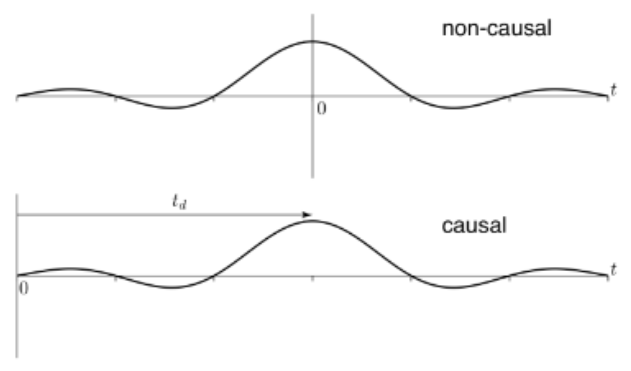
\includegraphics[width=\textwidth]{W8_1.png}
\end{center}
\subsection*{Distortionless LTI Systems}
When using filters, distortion could be introduced.  In the frequency domain, depending on the filter being used, components of the signal at different frequencies may be amplified differently or may be delayed.  We know that filtering causes:
\begin{itemize}
    \item Amplitude scaling by $|H(j\omega)|$
    \item Phase shifting by $\angle H(j\omega)$
\end{itemize}
and depending on the frequencies of the signal, this could cause distortion to the system.\\\\
A system is without distortion if
\[y(t) = Kx(t - t_d)\]
where $K$ is a scaling factor and $t_d$ is a delay.  This tells us that a distortionless signal is one that is identical to the input signal up to amplification and a constant delay.\\\\
What is $H(j\omega)$ for a distortionless LTI system?\\\\
This is a system with 
\[|H(j\omega)| = K\]
and
\[\angle H(j\omega) = -\omega t_d\]
It has the following amplitude and phase spectra:
\begin{center}
    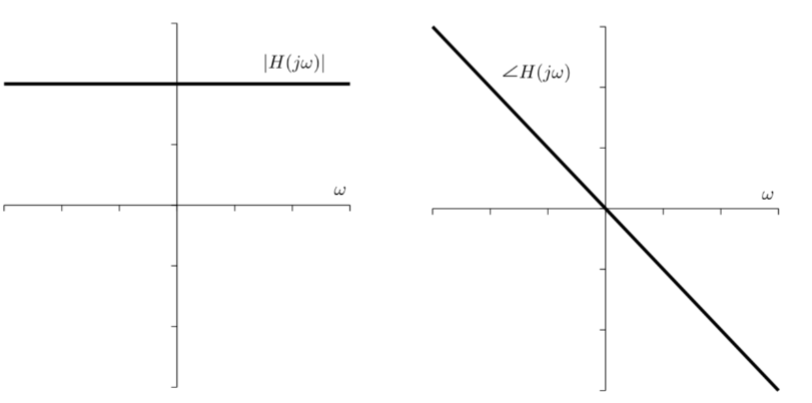
\includegraphics[scale=0.5]{W8_2.png}
\end{center}
\subsection*{Amplitude Distortion}
Amplitude distortion is relatively straightforward.
\begin{center}
    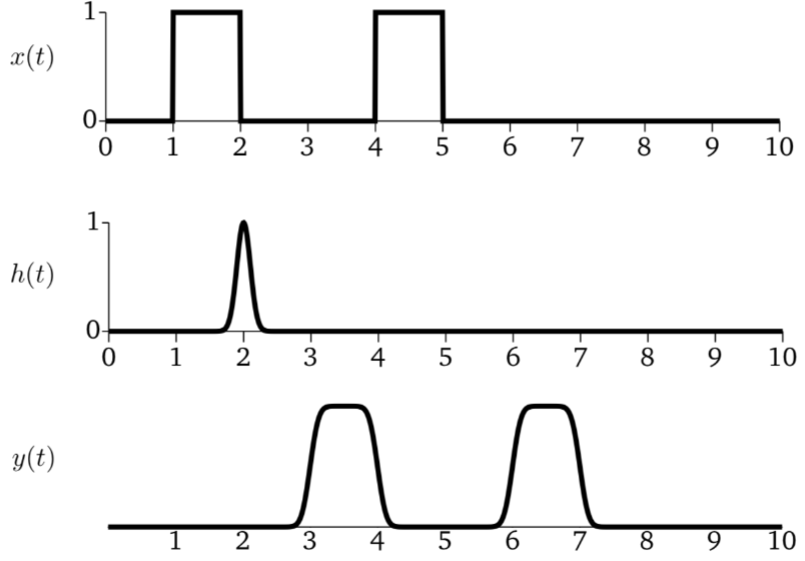
\includegraphics[scale=0.5]{W8_3.png}
\end{center}
If we have an impulse which is not really an impulse (due to real life physics limitations), we get some distortion in the output.
\subsection*{Phase Distortion}
\begin{center}
    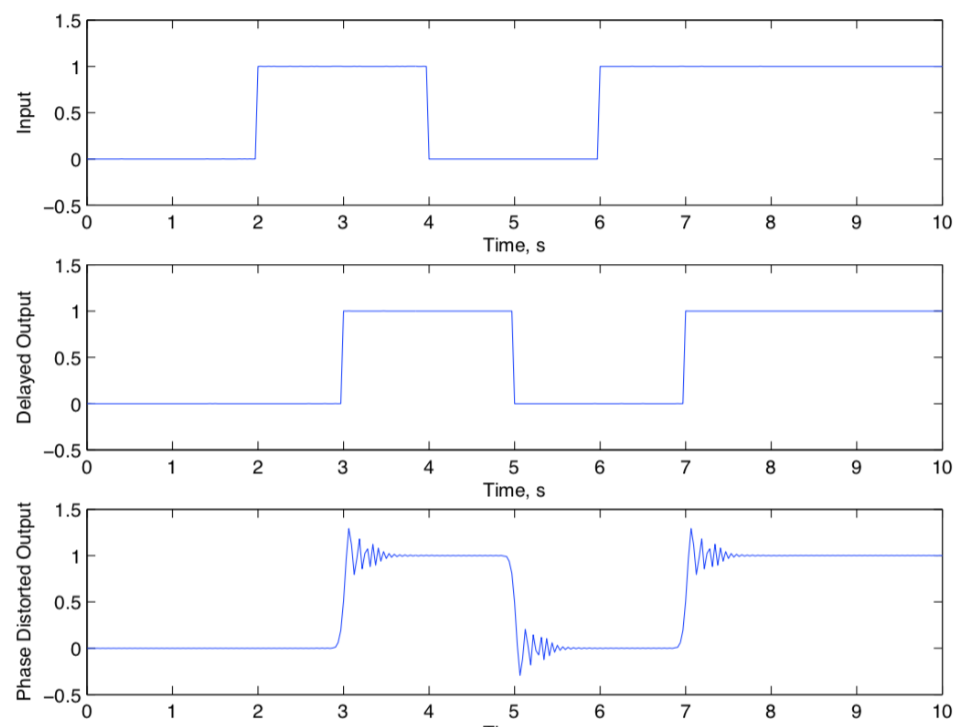
\includegraphics[scale=0.8]{W8_4.png}
\end{center}
\begin{itemize}
    \item Phase distortion is caused when the different complex exponentials that compose a function are changed by slightly different frequencies, so when they sum together, something weird happens.
    \item Think: Suppose $\angle(Y(j\omega)) = \angle(x(j\omega)) + \angle(h(j\omega))$.  If a distortion in phase is made to both $x$ and $h$, does $Y$ move by the same amount?  Especially with a frequency change, they may not line up well. 
\end{itemize}
\subsection*{Group Delay}
We know that convolution with $\delta(t - t_d)$ only delays the signal, but introduces no distortion.  Further, $\fourier[\delta(t - t_d)] = e^{-j\omega t_d}$, and so its phase is
\[\angle H(j\omega) = -\omega t_d\]
It turns out that if the phase is linear, the signal is only delayed in time without distortion.\\\\
Consider a simple example, a signal $x(t) = \cos(\omega t) + \cos(2\omega t)$.  Delaying this signal by $\pi / \omega$, i.e., $y(t) = x(t) * \delta(t - \pi - \omega)$ gives
\begin{align*}
    y(t) &= \cos(\omega(t - \pi/\omega)) + \cos(2\omega(t - \pi / \omega))\\
    &= \cos(\omega t - \pi) + \cos(2\omega t - 2\pi)
\end{align*}
This makes intuitive sense, if the signal is higher frequency, we need a larger phase shift to gain the same temporal offset.\\\\
When the phase is not linear, different frequencies will experience different temporal delays.  Therefore, the amount of delay will be frequency dependent, i.e., $t_d$ will be a function of $\omega$.  Since $\angle H(j\omega) = -\omega t_d$, it is straightforward to derive what the frequency-dependent temporal delay is, i.e., it's
\[t_d(\omega) = -\frac{\dd}{\dd \omega} \angle H(j\omega)\]
From this, we can see that if $\angle H(j\omega)$ is a line with slope $-k$, then its derivative is simply $-k$, leading to every frequency having the same delay $t_d = k$.  This confirms our intuition from before.\\\\
This quantity, $t_d(\omega)$, is called \textit{group delay}.
\subsection*{Distortions}
Importance of amplitude and phase distortion depends on application.\\\\
For audio or speech:
\begin{itemize}
    \item Amplitude distortion is very is important.
    \item Humans are relatively insensitive to phase distortion.
\end{itemize}
For images or video:
\begin{itemize}
    \item Amplitude distortion is relatively unimportant, as long as it is slowly varying.
    \item Phase distortion is very important.  Small amounts of non-linear phase result in very blurry looking images.
\end{itemize}
\section*{Sampling}
\subsection*{Motivation}
In reality, we could never store a continuous time signal.  Instead, as we see in \texttt{MATLAB}, we store a signal's value at various times.\\\\
A key variable of interest is the sampling frequency, i.e., the time in between our samples, denoted $T$ in the above diagram.\\\\
This is related to discrete signals, i.e., $x[n] = x(nT)$.
\subsection*{How to sample a continuous signal?}
How do we sample a continuous signal?  You may have several intuitions to do so already using the $\delta(t)$ signal and its property that $f(t) \delta(t) = f(0) \delta(t)$.
\begin{itemize}
    \item We will arrive at sampling by first studying a related problem: the Fourier transform of periodic signals.
    \item The reason we approach this is that Fourier series are discrete coefficients, $c_k$, while the Fourier transform is typically some continuous signal.  i.e., it seems like there may be a relationship whereby the Fourier series is like a sampled Fourier transform.
    \item So we ask: what is the relationship between the Fourier series and the Fourier transform?
    \item To see this, we can begin by identifying the relationship between the Fourier series and the Fourier transform.
\end{itemize}
\subsection*{Fourier transform of a periodic signal}
We cannot directly take the Fourier transform of a periodic signal, since they do not have finite energy.  However, we can use a few tricks (like in the Generalized Fourier Transform lecture) to calculate the FT of a periodic signal.\\\\
Let $f(t)$ have a Fourier series (with period $T_0 = \omega_0/2\pi$)
\[f(t) = \sum_{k = -\infty}^\infty c_k e^{jk\omega_0 t}\]
with 
\[c_k = \frac{1}{T_0} \int_{0}^{T_0} f(t) e^{jk\omega_0 t} \dd t\]
There's a close relationship between the two, as the Fourier series equation looks like the Fourier transform equation but with a $\sum$ instead of an $\int$.
\begin{center}
    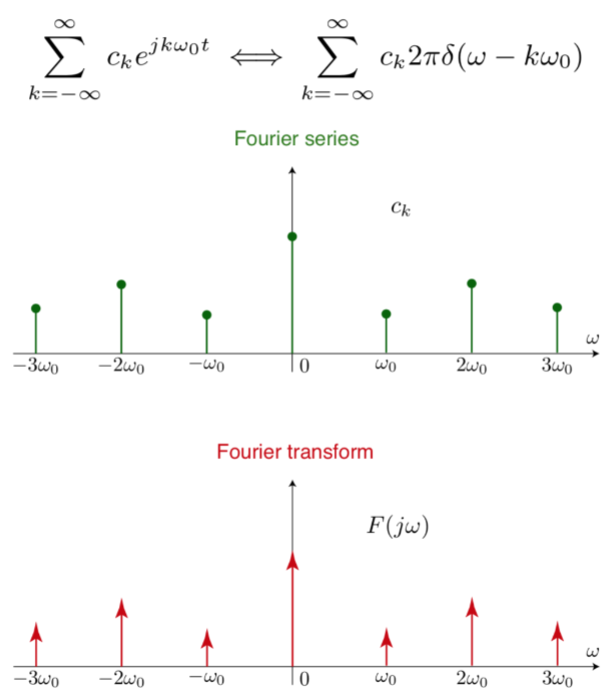
\includegraphics[scale=0.6]{W8_5.png}
\end{center}
\example\\
Consider the square wave below:
\[f(t) = \sum_{k=-\infty}^\infty \rect(t - 2k)\]
This is illustrated below:
\begin{center}
    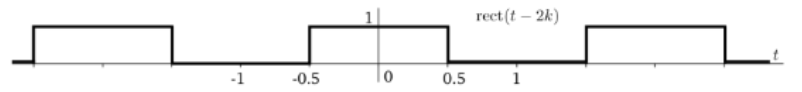
\includegraphics[width=\textwidth]{W8_6.png}
\end{center}
In the Fourier series lecture (slides 8-32), we calculated that the Fourier series of this signal is:
\[c_k = \frac{1}{2}\sinc(k/2)\]
What is its Fourier transform?
\[\sum_{k=-\infty}^\infty c_k e^{jk\omega_0 t} \llra \sum_{k=-\infty}^\infty c_k 2\pi \delta(\omega - k\omega_0)\]
\[F(j\omega) = \sum_{k=-\infty}^\infty \frac{1}{2} \sinc\left(\frac{k}{2}\right) \cdot 2\pi \cdot \delta(\omega - k\pi)\]
The $\delta(\omega - k\pi)$ is an impulse at $\omega = k\pi$.  Therefore, $k = \frac{\omega}{\pi}$.\\\\
Hence, the Fourier transform of the square wave is the Fourier transform of a $\rect$ multiplied by evenly spaced $\delta$'s, i.e.,
\begin{align*}
    F(j\omega) &= \pi \sum_{k=-\infty}^\infty \sinc(\omega/2\pi) \delta(\omega - k\pi)\\
    &= \pi \cdot \sinc(\omega/2\pi) \cdot \sum_{k=-\infty}^\infty \delta(\omega - k\pi)\\
\intertext{Impulse train notation: (this is discussed below.)}
    &= \pi \cdot \sinc\left(\frac{\omega}{2\pi}\right) \cdot \delta_\pi(\omega)
\end{align*}
\begin{center}
    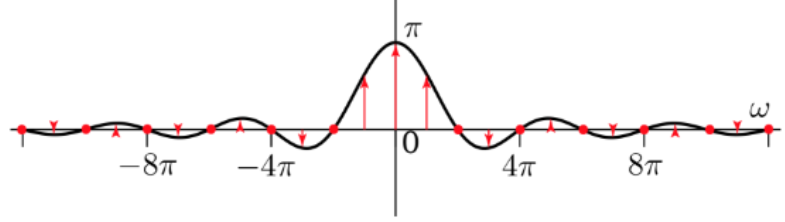
\includegraphics[width=\textwidth]{W8_7.png}
\end{center}
\subsubsection*{Impulse Trains}
To simplify the notation here, we can define an \textit{impulse train} which ends up being our sampling function.  We let $\delta_T(t)$ be a sequence of unit $\delta$ functions spaced by $T$.
\[\delta_T(t) = \sum_{k=-\infty}^\infty \delta(t - kT)\]
This is illustrated below:
\begin{center}
    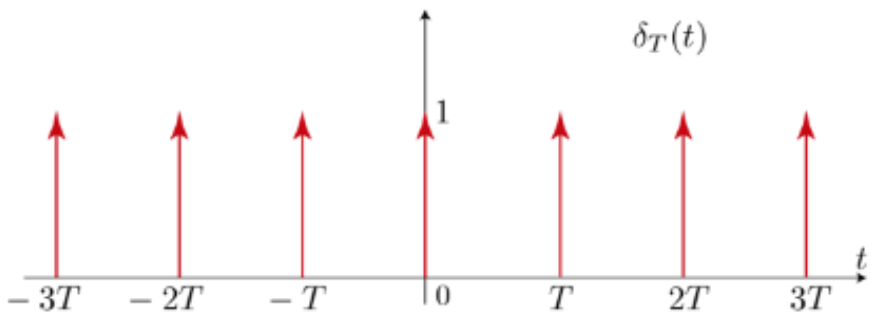
\includegraphics[width=\textwidth]{W8_8.png}
\end{center}
\subsection*{Fourier Series of Impulse Train}
By intuition:
\begin{itemize}
    \item We know that the Fourier transform of the square wave is a $\sinc$ multiplied by a $\delta_\pi(\omega)$.
    \item From the convolution theorem, this means that the inverse Fourier transform (i.e., the square wave) is the inverse Fourier transform of a $\sinc$ convolved with the inverse Fourier transform of a impulse train.
    \item We know that a square is simply a $\rect$ repeated over and over again, i.e., convoluted with a impulse train.
    \item So intuitively, the Fourier transform of a impulse train should be a impulse train.
    \item Note: we will sometimes use the term 'delta train' to describe an impulse train.
\end{itemize}
Proof:
\begin{align*}
    c_k &= \frac{1}{T} \int_{\text{1 period}} f(t) e^{-jk\omega_0 t} \dd t\\
    &= \frac{1}{T} \int_{-\frac{T}{2}}^{\frac{T}{2}} \delta_T(t) \cdot e^{-jk\omega_0 t} \dd t\\
    \intertext{Note that $\omega_0 = 2\pi/T$}
    &= \frac{1}{T} \int_{-\frac{T}{2}}^{\frac{T}{2}} \delta(t) e^0 \dd t\\
    \Aboxed{c_k &= \frac{1}{T}}
\end{align*}
Therefore,
\begin{align*}
    \fourier[\delta_T(t)] &= \fourier\left[\frac{1}{T} \sum_{k=-\infty}^\infty e^{jk\omega_0 t}\right]\\
    &= \frac{1}{T} \sum_{k=-\infty}^\infty \fourier\left[e^{-jk\omega_0 t}\right]\\
    \intertext{Recall that $e^{jk\omega_0 t} \llra 2\pi \cdot \delta(\omega - k\omega_0)$.}
    &= \frac{1}{T} \sum_{k=-\infty}^\infty 2\pi \cdot \delta(\omega - k\omega_0)\\
    &= \omega_0 \cdot \delta_{\omega_0}(\omega)
\end{align*}
By this, the Fourier transform of an impulse train is an impulse train.
\subsection*{Sampling with an impulse train}
As we saw earlier, one of the things we will use the impulse train for is to sample signals.\\\\
Given a signal $f(t)$,
\begin{align*}
    f(t) \delta_T(t) &= f(t) \cdot \sum_{k=-\infty}^\infty \delta(t - kT)\\
    &= \sum_{k=-\infty}^\infty f(t) \cdot \delta(t - kT)\\
    \Aboxed{\hat{f}(t) &= \sum_{k=-\infty}^\infty f(kT) \cdot \delta(t - kT)}
\end{align*}
\subsection*{Square Wave Example pt. 2}
Let's revisit our square wave example, where
\[f(t) = \sum_{k=-\infty}^\infty \rect(t-2k)\]
Another way to represent this square wave is as follows:
\[f(t) = \rect(t) * \delta_2(t)\]
Hence, we can calculate its Fourier transform by using the convolution theorem.  Recall that, for $\omega_0 = 2\pi/T$.
\[\rect(t) \llra \sinc(\omega/2\pi)\]
and
\[\delta_T(t) \llra \omega_0 \delta_{\omega_0} (\omega)\]
Note that when $T = 2$, then $\omega_0 = \pi$.  Then, we have that,
\begin{align*}
    \fourier[f(t)] &= \fourier[\rect(t) * \delta_2(t)]\\
    &= \fourier[\rect(t)] \fourier[\delta_2(t)]\\
    &= \sinc(\omega/2\pi) \pi \delta_\pi(\omega)
\end{align*}
This is exactly the same Fourier transform we calculated earlier using the Fourier series of the square wave.
\subsection*{Sampling and Periodicity}
Another intuition to remember here is that the Fourier transform of a periodic signal is the Fourier transform of one period of the signal (which we can denote $f_1$), sampled by an impulse train at multiples of $\omega_0$.
\begin{center}
    \includegraphics*[width=\textwidth]{W8_9.png}
\end{center}
\textbf{Discrete (sampling) - periodic duality}\\\\
We can determine the Fourier transform of a signal sampled in the time domain.  Consider
\[\tilde{f}(t) = f(t) \delta_T(t)\]
Its Fourier transform is
\[\tilde{F}(j\omega) = \fourier[f(t) \delta_T(t)]\]
These are merely samples of $F(j\omega)$ repeated every $\omega_0$, since
\begin{align*}
    \tilde{F}(j\omega) &= \frac{1}{T} F(j\omega) * \delta_{\omega_0}(\omega)\\
    &= \frac{1}{T} F(j\omega) * \sum_{k=-\infty}^\infty \delta(\omega - k\omega_0)\\
    &= \frac{1}{T} \sum_{-\infty}^\infty F(j(\omega - k\omega_0))
\end{align*}
This leads us to the realization that:
\begin{itemize}
    \item A signal that is periodic in time is \textbf{sampled} in spectrum.
    \item A signal that is sampled in time is \textbf{periodic} in spectrum.
\end{itemize}
There are important consequences from this result when we consider sampling signals in the time domain.

\subsection*{Sampling Theorem}
Consider the following problem.  We have a signal $f(t)$, and we need to store it.  Our experimental set up is able to sample this signal at an interval $T$.  How do we set $T$ so that we can faithfully store $f(t)$.  If $T$ is too large, we sample infrequently and may lose information about $f(t)$.  If $T$ is too small, we waste memory and resources to store values we don't need.\\\\
The sampling theorem uses the results we've derived to tell us the minimum frequency at which we must sample $f(t)$ to not lose information.  It is a very important theorem.\\\\
If $\tilde{f}(t) = f(t) \delta_T(t)$, then 
\[\tilde{F}(j\omega) = \frac{1}{T} \sum_{k=-\infty}^\infty F(j(\omega - k\omega_0))\]
Therefore, the spectrum of $\tilde{f}(t)$ are shifted replicas of the spectrum, $F(j\omega) = \fourier[f(t)]$ spaced every $\omega_0$ and scaled by $1/T$.  We define the bandwidth of $f(t)$ to be $\pm B$ Hz, e.g.,
\begin{center}
    \includegraphics*[width=\textwidth]{W8_10.png}
\end{center}
For a particular choice of $\omega_0$, where $\omega_0 \gg 2\pi B$, we see the spectrum of $\tilde{F}(j\omega)$ looks like:
\begin{center}
    \includegraphics*[scale=0.8]{W8_11.png}
\end{center}
For this choice of $\omega_0$, the original $F(j\omega)$ can be recovered through low pass filtering.
\begin{itemize}
    \item This is because the triangles are not overlapping.
\end{itemize}
With ideal low pass filtering for the illustrated $\omega_0$, we can \textit{perfectly} recover $f(t)$ after sampling.\\\\
However, if we increase the time $T$ between samples, which decreases $\omega_0$, the replicas of $F(j\omega)$ get closer and closer together.
\begin{center}
    \includegraphics*[scale=0.8]{W8_12.png}
\end{center}
We can see that as $\omega_0$ decreases, the bands start to overlap.  When the replicas overlap, even with ideal low pass filtering, we cannot recover the original $F(j\omega)$.\\\\
This overlap is called \textit{aliasing} because low frequencies of one spectral replica appear (or alias) as high frequencies in the next spectral replica.  The vice versa is true as well; high frequencies of one spectral replica alias as low frequencies in an adjacent spectral replica.  The aliased sections are shown in the darker red.
\begin{center}
    \includegraphics*[scale=0.8]{W8_13.png}
\end{center}
To perfectly recover a signal, we need to sample so as to avoid aliasing.  No aliasing happens if $2\pi B < \omega_0 / 2$.  We can simplify this as
\begin{align*}
    2B &< \omega_0 / 2\pi\\
    &= \frac{2\pi}{T} \frac{1}{2\pi}\\
    &= \frac{1}{T}
\end{align*}
Therefore, the signal can only be recovered exactly if the signal bandwidth $2B$ is less than or equal to the sampling rate $1/T$.  Hence, we need to sample at intervals less than or equal to $T = 2B$.  This sampling rate, $2B$ is called the \textit{Nyquist rate} for $f(t)$, and it is the lowest rate that we can sample $f(t)$ so that it can be perfectly recovered.  $T$ is called the \textit{Nyquist Interval}.

\subsection*{Recovering the original signal through Interpolation}
With a sampled signal, $\tilde{f}(t)$, as long as we have sampled at a rate $\geq 2B$, we can perfectly recover the original signal through ideal low pass filtering.  Let's formalize how this happens, using the particular instantiation that $T = \frac{1}{2}B$, i.e., we sample at the Nyquist rate.
\begin{center}
    \includegraphics*[scale=0.8]{W8_14.png}
\end{center}
Our low pass filter has frequency response
\[H(j\omega) = T\rect\left(\frac{\omega}{4B}\right)\]
The inverse Fourier transform of $H(j\omega)$ is:
\[h(t) = 2BT\sinc(2Bt)\]
Since $T = \frac{1}{2}B$, we can simplify this expression to 
\[h(t) = \sinc(2Bt)\]
Therefore, to reconstruct $f(t)$ from $\tilde{f}(t)$, we calculate:
\begin{align*}
    \tilde{f}(t) * h(t) &= \left(\sum_{k=-\infty}^\infty f(kT) \delta(t - kT)\right) * h(t)\\
    &= \sum_{k=-\infty}^\infty f(kT) h(t - kT)\\
    &= \sum_{k=-\infty}^\infty f(kT) \sinc(2B(t-kT))\\
    &= \sum_{k=-\infty}^\infty f(kT) \sinc(2Bt - k)
\end{align*}
This reconstruction,
\[\boxed{\tilde{f}(t) * h(t) = \sum_{k=-\infty}^\infty f(kT) \:\sinc(2Bt - k)}\]
is called the \textbf{Whittaker-Shannon interpolation formula}.  Intuitively, it does the following:
\begin{center}
    \includegraphics*[width=\textwidth]{W8_15.png}
    \includegraphics*[width=\textwidth]{W8_16.png}
\end{center}
The sum of the green sinc functions will equal the red function, $f(t)$.\\\\
To not mince words, this result is remarkable.  Through this reconstruction, we are able to \textit{perfectly} recover an original signal from samples.

\subsection*{Example: Sinusoids}
Let's consider sampling a cosine,
\[f(t) = \cos(\omega_0 t)\]
Let's take $\omega_0 = 2\pi$.  What is B?
[FILL]

\subsection*{Aliasing Example}
Here's an example of aliasing.  Below are two sinusoids.  The upper one is at a frequency of $f=0.75$ Hz and the one below is at $f = 1.25$ Hz.\\\\
Sampling both signals at $f_s = 2$ Hz,
\begin{center}
    \includegraphics*[scale=0.8]{W8_17.png}
\end{center}
As you can see, the samples are the same for both sinusoids, however the sampling is below the nyquist rate of the bottom function (and equal to the nyquist rate of the top function).\\\\
Using these points for reconstruction will yield the $f=0.75$ Hz sinusoid.

\subsubsection*{Looking at aliasing in the Frequency Domain}
\begin{center}
    \includegraphics*[scale=0.7]{W8_18.png}
\end{center}
The top set corresponds to the top cosine wave ($f = 0.75$), and the bottom set corresponds to the bottom cosine wave ($f=1.25$)

\subsection*{How to ameliorate aliasing}
If you sample below the Nyquist rate, there will be aliasing.  Once aliasing happens, there is no way to eliminate aliasing without having additional information about the signal.\\\\
One way we can ameliorate aliasing is to first low pass filter the signal, then sample.
\begin{center}
    \includegraphics*[scale=0.8]{W8_19.png}
\end{center}
\begin{itemize}
    \item In reality, our low pass filters are not perfect, and so the bandwidth will be larger than $\omega_0 / 2$.  However, we'll attenuate frequencies outside of range.
    \item Low pass filtering will distort the signal.
    \item However, the point is that when sampling, frequencies beyond $\omega_0 / 2$ would cause artifacts.  Low pass filtering ameliorates this.
    \item It also supresses noise outside of $\omega_0 / 2$.
\end{itemize}

\section*{Laplace Transform}
\textbf{Motivation:}
The Fourier transform is powerful, but it doesn't exist for some signals and systems. In several applications, including image processing, communications, and circuit design, its sufficient for analysis.\\\\
However, some systems are unstable, or are power signals where the Fourier transform can not be straightforwardly generalized. Some examples of this are signals that grow with time, like (ideally) your bank account, or the S\&P 500.\\\\
How do we analyze these systems in a similar framework to what Fourier analysis enables us to do?

\subsection*{Motivating Example}
Let
\[f(t) = e^{at} u(t)\]
When $a > 1$, this signal does not have a Fourier transform.\\\\
One approach to arrive at a Fourier transform is to define a new function
\[g(t) = f(t) e^{-\sigma t}\]
If $\sigma > a$, then $g(t)$ is a decreasing exponential, which has a Fourier transform.\\\\
The function $g(t) = f(t) e^{-\sigma t}$ has a Fourier transform for $\sigma$ sufficiently large.  The Fourier transform of $g(t)$ comprises how to sum spectral components of $e^{j\omega t}$,
\[g(t) = \frac{1}{2\pi} \absint G(j\omega) e^{j\omega t} \dd \omega\] 
The intuition here is that because $f(t) = g(t) e^{\sigma t}$, $f(t)$ has spectral components
\[e^{\sigma t} e^{j\omega t} = e^{(\sigma + j\omega)t}\]
Hence, the Laplace transform gives us a spectrum of $f(t)$ in terms of a complex exponential with both real and imaginary components (where as the Fourier transform was only with imaginary components.)
\begin{center}
    \includegraphics*[scale=0.8]{W8_20.png}
\end{center}
\subsubsection*{When does the $s$-spectrum exist?}
For what values fo $\sigma$ does this work?  In the case where $f(t) = e^{at} u(t)$, this is clear, i.e., $\sigma > a$.\\\\
In general, there is some $\sigma_0$ for which
\[f(t) e^{-\sigma_0 t}\]
goes to zero.  If it does, then this $f(t) e^{-\sigma_0 t}$ is an energy signal, and its spectrum will exist.  The portion of the complex plane where $\sigma > \sigma_0$ is called the "region of convergence".\\\\
This is illustrated below:
\begin{center}
    \includegraphics*[scale=0.8]{W8_21.png}
\end{center}
Note that the $y$-axis on this graph is when $s = j\omega$, and $\sigma = 0$.  This is the Fourier transform.\\\\
The region of convergence is where $s = \sigma + j\omega$.  Note that the region of convergence does not include the $j\omega$ axis.\\\\
For a function to have a valid Fourier transform, its region of convergence MUST include the axis.

\subsection*{Laplace transform notation}
Our notation for the Laplace transform is very similar to our prior notation.  We denote
\begin{align*}
    F(s) &= \mathcal{L}[f(t)]\\
    f(t) &= \mathcal{L}^{-1}[F(s)]
\end{align*}
We will also denote this:
\[f(t) \llra F(s)\]
Remember that $s = \sigma + j\omega$.


\subsection*{Bilateral Laplace Transform (Not on exam)}
The Laplace transform incorporates the real exponential.  With $s = \sigma + j\omega$, as before, 
\begin{itemize}
    \item $j\omega$ is related to the oscillatory component of the complex exponential
    \item $\sigma$ is related to the decay or growth of the complex exponential
\end{itemize}
Then, the \textbf{bilateral} Laplace transform is:
\[\boxed{F(s) = \absint f(t) e^{-st} \dd t}\]
To invert the bilateral Laplace transform, we calculate:
\[\boxed{f(t) = \frac{1}{2\pi j} \int_{c - j\omega}^{c + j\omega} F(s) e^{st} \dd s}\]
for $c > \sigma_0$.

\subsection*{Unilateral Laplace Transform}
Usually, we are interested in analyzing causal signals.  In this case, we can simplify the bilateral Laplace transform.  A causal signal can be written as $f(t)u(t)$, and its Laplace transform is
\begin{align*}
    F(s) &= \absint f(t)u(t) e^{-st} \dd t\\
    &= \int_{0^-}^\infty f(t) e^{st} \dd t
\end{align*}
When we write $0^-$, this indicates that impulses at the origin are included (e.g., $\delta(t)$ would have a contribution to this integral).\\\\
The Laplace transform is (essentially) unique.  From now on, we'll use $\laplace[f(t)]$ to denote the unilateral Laplace transform of $f(t)$.

\subsection*{Laplace Transform Properties}
\begin{enumerate}[label=\arabic*.]
    \item \textbf{Linearity:}
    \[\boxed{\laplace[af_1(t) + bf_2(t)] = aF_1(s) + bF_2(s)}\]
    \item \textbf{Time scaling:}
    \[\boxed{\laplace[f(at)] = \frac{1}{a} F\left(\frac{s}{a}\right)}\]
    \item \textbf{Time shift:}
    \[\boxed{\laplace[f(t - T)] = e^{-sT} F(s)}\]
    \item \textbf{Frequency shift:}
    \[\boxed{\laplace[f(t) e^{s_0 t} = F(s - s_0)]}\]
    \item \textbf{Convolution:}
    \[\boxed{\laplace[f_1(t) * f_2(t) = F_1(s) F_2(s)]}\]
    \item \textbf{Integration:}
    \[\boxed{\laplace\left[\int_0^t f(\tau) \dd \tau\right] = \frac{1}{s} F(s)}\]
    \item \textbf{Derivative:}
    \[\boxed{\laplace[f'(t)] = sF(s) - f(0)}\]
    \item \textbf{Multiplication by $t$:}
    \[\boxed{\laplace[t f(t)] = -F'(s)}\]
\end{enumerate}
\subsection*{Relationship between the Fourier and Laplace transforms}
The Fourier transform is a special case of the Laplace transform, i.e.,
\[\boxed{F(j\omega) = F(s) \vert_{s=j\omega}}\]
The Fourier transform is evaluated at $s = j\omega$ and the Laplace transform is evaluated at a particular $s = \sigma + j\omega$.
\begin{center}
    \includegraphics*[scale=0.7]{W8_22.png}
\end{center}
You may imagine that for signals where we know the Fourier transform, the Laplace transform merely replaces $j\omega$ with $s$.  This is sometimes the case.  Let's consider $f(t) = e^{-at} u(t)$.
\begin{align*}
    F(s) &= \int_0^\infty e^{at} e^{-st} \dd t\\
    &= \int_0^\infty e^{-(a + s)t} \dd t\\
    &= \left.-\frac{1}{a + s} e^{-(a + s)t}\right|_0^\infty\\
    &= \frac{1}{a + s}
\end{align*}
As long as $e^{-(a + s)t} \rightarrow 0$ as $t \rightarrow \infty$.  When does this happen?\\\\
If $e^{-(a+s)t}$ goes to zero, then so does $|e^{-(a+s)t}|$.
\begin{align*}
    |e^{-(a+s)t}| &= |e^{-(a + \sigma + j\omega)t}|\\
    &= |e^{-(a+\sigma)t} \cdot e^{-j\omega t}|\\
    &= |e^{-(a+\sigma)t}| \cdot |e^{-j\omega t}|\\
    \intertext{(Fourier transform $e^{-j\omega t}$ evaluates to 1\dots)}
    &= |e^{-(a+\sigma)t}|
\end{align*}
Therefore, $e^{-(a+s) t} \rightarrow 0$ if $e^{-(a + \sigma)t} \rightarrow 0$ as $t \rightarrow \infty$.\\\\
If $\sigma > -a$, then the Laplace transform exists.
\[\boxed{\text{Rate of Change:  } \sigma = \text{Re}(s) > -a}\]
Hence, we have that
\[\laplace[e^{-at} u(t)] = \frac{1}{a + s}\]
and we know prior, for $a > 0$,
\[\fourier[e^{-at} u(t)] = \frac{1}{a + j\omega}\]
Here, the Laplace transform is the Fourier transform, with $j\omega$ replaced with $s$.\\\\
A key thing to note is that with 
\[\laplace[e^{-at} u(t)] = \frac{1}{a + s}\]
holds for all $a$, positive or negavie, as long as $\sigma > -a$.  This means that, for all $a > 0$, 
\[\laplace[e^{at} u(t)] = \frac{1}{s - a}\]
Of course, this signal does not have a Fourier transform.


\end{document}